\documentclass[12pt, french]{article}

\usepackage{fancyhdr, fancybox, lastpage,mhchem, mathrsfs, tikz}
\usepackage[most]{tcolorbox}
\usepackage[a4paper, margin={0.3in, .75in}]{geometry}
\usepackage{wrapfig}
\pagestyle{fancy}
\renewcommand\headrulewidth{1pt}
\renewcommand\footrulewidth{1pt}
\fancyhf{}
\rhead{ \em{Zakaria Haouzan}}
\lhead[C]{\em{2ème année baccalauréat Sciences Physiques}}
\chead[C]{}
\rfoot[C]{}
\lfoot[R]{}
\cfoot[]{\em{Page \thepage / \pageref{LastPage}}}


\newtcolorbox{Box2}[2][
enhanced, 
    breakable,
]{
                lower separated=false,
                colback=white,
colframe=white!20!black,fonttitle=\bfseries,
colbacktitle=white!30!gray,
coltitle=black,
enhanced,
attach boxed title to top left={yshift=-0.1in,xshift=0.15in},
title=#2,#1}


\begin{document}
\begin{center}
   \shadowbox {\bf{Mouvement d’un projectile dans un champ de pesanteur
uniforme}
 }

\end{center}

\vspace{-0.2cm}
%%_________________________Exercice ! :"_________________________Exercice
   \begin{Box2}{Exercice 1 : Étude du mouvement d'un solide dans le champ de pesanteur uniforme}

	\begin{wrapfigure}[4]{r}{0.32\textwidth}
  \begin{center}
	  \vspace{-0.6cm}
	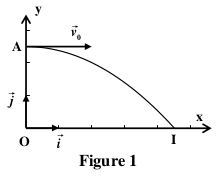
\includegraphics[width=0.32\textwidth]{./ex_00_0.png}
  \end{center}
\end{wrapfigure}

 
% Required package
On lance, à un instant t0 = 0 avec une vitesse initiale $\vec{v_0}$
 horizontale, un solide (S) de petites dimensions, de masse m , d'un
point A qui se trouve à la hauteur h du sol. Le solide (S) tombe
sur le sol au point d'impact I (figure 1).
On étudie le mouvement du centre d'inertie G dans le repère $(O,\vec{i}, \vec{j})$ lié à la terre supposé galiléen.

\textbf{Données:}
\begin{itemize}
\item Tous les frottements sont négligeables;
\item $g = 9,8 m.s^{-2}$ ; $h = OA= 1 m$
\end{itemize}

\begin{enumerate}
	\item En appliquant la deuxième loi de Newton, établir les expressions littérales des équations horaires
x(t) et y(t) du mouvement de G .
\item En déduire l'expression littérale de l'équation de la trajectoire du mouvement de G .
\item Calculer la valeur de $t_I$ , l'instant d'arrivé de (S) au sol en I .
\item On lance de nouveau, à un instant $t_0 = 0$ , le solide (S) du point A avec une vitesse initiale
$\vec{v'_0} = 3.\vec{v_0}$.

Recopier sur votre copie le numéro de la question et écrire la lettre correspondante à la seule
proposition vraie:
la valeur de l'instant d'arrivé de (S) au sol vaut:

a) $t' = 0,25s$ \hspace{3cm} b)$t' = 0,35s$ \hspace{2cm} c)$t' = 0,45s$ \hspace{2cm} d)$t'=0,65s$

\end{enumerate}

   \end{Box2}


%%_________________________Exercice !2 :"_________________________Exercice
\begin{Box2}{Exercice 2 :Mouvement du système (S) durant la phase du saut }
   % \begin{wrapfigure}[6]{r}{0.32\textwidth}
  %\begin{center}
	  %\vspace{-0.6cm}
	%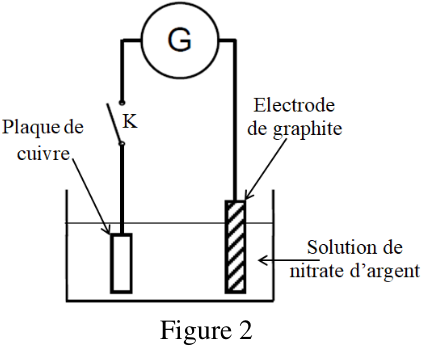
\includegraphics[width=0.32\textwidth]{./ex_01.png}
  %\end{center}
%\end{wrapfigure}

	\emph{Le saut en longueur avec moto est considéré parmi les sports motivant, attirant et défiant pour
dépasser certains obstacles naturels et artificiels.
Le but de cet exercice est d’étudier le mouvement du centre d’inertie G d’un système (S) de
masse m constitué d’une moto avec motard sur une piste de course.}

La piste de course est constituée d’une partie rectiligne horizontale, d’une partie rectiligne inclinée d’un
angle $\alpha$ par rapport au plan horizontal et d’une zone de chute comportant un obstacle (E) de
hauteur L situé à la distance d de l’axe vertical passant par le point D , (fig1).

\begin{center}
	%\vspace{-0.6cm}
	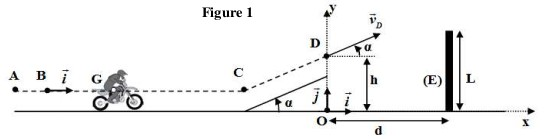
\includegraphics[width=0.72\textwidth]{./ex_01_00.jpg}
  \end{center}

	\vspace{-1.8cm}
\textbf{Données:}
\begin{itemize}
	\item Tous les frottements sont négligeables ;
	\item  $d=20m$ ; $L=10m$ ; $\alpha = 26^{\circ}$ ; $m=190Kg$
\end{itemize}
Le système (S) quitte la piste de course au passage de G par le point D avec une vitesse $v_D$ formant un
angle $\alpha$ avec le plan horizontal pour sauter à travers l’obstacle (E) (voir fig. (1)). Au cours du saut le
système (S) n’est soumis qu’à son poids.

On étudie le mouvement de G dans le champ de pesanteur uniforme dans un repère orthonormé
$(O.\vec{i}.\vec{j})$ lié à la terre considéré comme galiléen. On choisit l’instant de passage de G par le point
D comme nouvelle origine des dates $t_0 = 0$ , tel que : $y_0 = OD = h$ .
\begin{enumerate}
	\item En appliquant la deuxième loi de newton, montrer que les équations différentielles vérifiées par $x_G (t)$ et $y_G (t)$ coordonnées de G dans le repère $(O.\vec{i}.\vec{j})$ sont : $$\frac{x_G}{dt} = v_D.\cos{\alpha} \hspace{3cm} \frac{y_G}{dt} = -g.t +v_D.\sin{\alpha}$$

	\item L’expression numérique des équations horaires xG (t) et yG (t) du mouvement de G est : $$x_G(t) = 22,5.t \hspace{1cm} (m) \hspace{3cm} y_G(t) = -5.t^2 +11.t + 5 \hspace{1cm} (m)$$
		Déterminer les valeurs de la hauteur h , et de la vitesse $v_D$.

	\item Le saut est réussi si la condition : $y_G > L+0,6$ (m) est vérifiée. Est-ce que le saut du motard est
réussi ? Justifier votre réponse.

\end{enumerate}




\end{Box2}

\begin{Box2}{Exercice 3 :Etude de la chute libre }

	\emph{Les hélicoptères sont parfois utilisés pour approvisionner, d’aides humanitaires, les
zones sinistrées non joignables par voies terrestres.}

	\begin{wrapfigure}[7]{r}{0.32\textwidth}
  \begin{center}

	  \vspace{-1.7cm}
	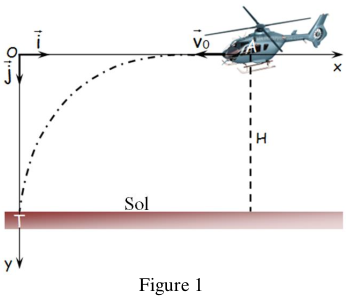
\includegraphics[width=0.32\textwidth]{./ex_02.png}
  \end{center}
\end{wrapfigure}
Un hélicoptère vole à une altitude H
constante par rapport au sol, avec une
vitesse horizontale $\vec{V_0}$ constante. Il
fait tomber un paquet d’aliments de
centre de gravité $G_0$, qui tombe sur le
sol au point T. (Figure 1)
On étudie le mouvement de G0 dans
un
repère
orthonormé $(R,O,\vec{i}, \vec{j})$
supposé galiléen.

\textbf{On donne :} $g = 10 m.s^{-2}$  ;  $H=405m$ ; On néglige les dimensions du paquet.

\textbf{\underline{Partie 1 : Etude de la chute libre : }}
On néglige les forces liées \\à l’action de l’air sur le paquet.
Le paquet tombe, à l’instant $t = 0$, à \\partir du point $A(x_A = 450 m, y_A = 0)$, avec une
vitesse initiale horizontale $\vec{V_0}$ de valeur $V_0 = 50 m.s^{-1}$.

\begin{enumerate}
	\item Par application de la deuxième loi de Newton, trouver les équations
		horaires x(t) et y(t) du mouvement de $G_0$ dans le repère $(R,O,\vec{i}, \vec{j})$.
	\item Déterminer l’instant d’arrivée du paquet au sol.
	\item  Trouver l’équation de la trajectoire du mouvement de $G_0$.
\end{enumerate}

\textbf{\underline{Partie 2 : Etude du mouvement du système (S) dans le champ de pesanteur uniforme: }}
Le système (S) arrive en O avec une vitesse $\vec{v_o}$ de module $v_0 =30 m.s^{ -1}$ , et poursuit son
mouvement pour tomber en E distant de C de la distance $CE = 43 m$.
On prendra comme instant du début du saut sur la tranchée comme nouvelle origine
des dates lorsque G coïncide avec O origine du repère $(\vec{Ox},\vec{Oz})$ (Figure 1).

\begin{enumerate}
	\item[4.]Ecrire les équations horaires x(t) et z(t) du mouvement de G dans $(\vec{Ox},\vec{Oz})$.
	\item[5.]  Déduire l’équation de la trajectoire et déterminer les coordonnées de son sommet.
	\item[6.] Déterminer la différence d’altitude h entre C et O.
\end{enumerate}

\end{Box2}
	%\vspace{-0.8cm}


\begin{Box2}{Exercice 4 :Les toboggans}
	\emph{Les toboggans dans les piscines permettent aux nageurs de glisser et de plonger
dans l’eau.
On modélise un toboggan par une piste ABC constituée d’une partie AB inclinée
d’un angle $\alpha$ par rapport au plan horizontal et d’une partie circulaire BC, et on
modélise le nageur par un solide (S) de centre d’inertie G et de masse m (Figure1). }
\textbf{Données:}$AB = 2,4 m$ , $\alpha$ = 20° , $g = 9,8 m.s^{-2}$ , $m = 70 Kg.$ 
	\begin{wrapfigure}[7]{r}{0.42\textwidth}
  \begin{center}

	  \vspace{-1.2cm}
	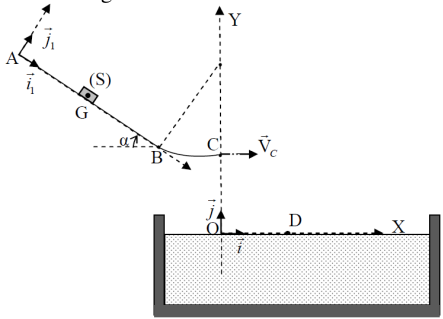
\includegraphics[width=0.42\textwidth]{./ex_03.png}
  \end{center}
\end{wrapfigure}

\textbf{\underline{Etude du mouvement de G dans l’air :}}

e solide (S) arrive au point C avec une
vitesse de vecteur horizontal, et de valeur
$V_C = 4,67 m.s^{-1}$, pour le quitter à un instant
supposé comme nouvelle origine des
temps.
Le solide est soumis, en plus de son poids,
à l’action d’une air artificielle, modélisée
par la force d’expression : $\vec{f_1}$=$ -f_1.\vec{i}$.

\begin{enumerate}
	\item Trouver, à un instant t, l’expression $v_x$ de la composante \\horizontale du
vecteur vitesse en fonction de : m, $V_C$, $f_1$, et t.

\item  A l’instant $t_D = 0,86 s$, G arrive au point D se trouvant à la surface de l’eau,
où s’annule la composante horizontale de sa vitesse.
\begin{enumerate}
	\item Calculer f1.
	\item Calculer l’altitude h de C par rapport à la surface de l’eau.
\end{enumerate}
\end{enumerate}

\end{Box2}




\begin{Box2}{Exercice 5 : Etude du mouvement du centre de gravité d’une balle. }

	\begin{wrapfigure}[12]{r}{0.42\textwidth}
  \begin{center}

	  %\vspace{-1.2cm}
	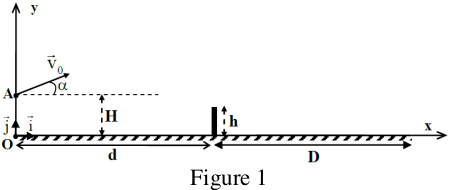
\includegraphics[width=0.42\textwidth]{./ex_04.png}
	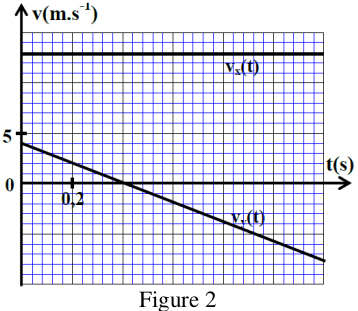
\includegraphics[width=0.39\textwidth]{./ex_04_0.png}
  \end{center}
\end{wrapfigure}


	Pendant un match de volley-ball, un élève a enregistré une séquence vidéo du
mouvement de la balle à partir de l’instant de l’exécution du service à partir d’un
point A situé à une hauteur H du sol. Le joueur ayant exécuté le service se trouve à
une distance d du filet (Figure 1).
Pour que le service soit bon, la balle doit vérifier les deux conditions suivantes :

\begin{itemize}
	\item Passer au-dessus du filet dont la partie supérieure se trouve à une hauteur h du sol ;
	\item Tomber dans le terrain de l’adversaire de longueur D.
	\item Données : On néglige les dimensions de la balle ainsi que l’action de l’air.
	\item On prendra l’intensité de la pesanteur : \\$g $=$10 m.s^{-2}$.
	\item $H = 2,60 m$ , $d = D = 9 m$ , $h = 2,50 m$.
\end{itemize}

On étudie le mouvement de la balle
dans un repère orthonormée $(O,\vec{i}, \vec{j})$
lié à la terre et supposé galiléen.
A l’instant $t = 0$, la balle se trouve
en A, et le vecteur vitesse initiale
$\vec{V_0}$ constitue l’angle $\alpha$ avec
l’horizontal. (Figure 1)
Un traitement informatique de la vidéo avec un logiciel convenable, a permis
d’obtenir les courbes représentées sur la figure 2.
Les courbes $v_x(t)$ et $v_y(t)$ représentent les variations des composantes du vecteur
vitesse du ballon dans le repère $(O,\vec{i}, \vec{j})$ .

\begin{enumerate}
\item Par application de la deuxième loi de
Newton, établir l’expression de $v_x(t)$ en
fonction de : $V_0$, $\alpha$, et l’expression de $v_y(t)$
en fonction de : $V_0$, $\alpha$, $g$ et $t$.

\item  En exploitant les deux courbes (Figure 2),
montrer que la valeur de la vitesse initiale
est $V_0 = 13,6 m.s^{-1}$, et que l’angle $\alpha$ est
$\alpha$=17°.

\item Etablir l’équation de la trajectoire de G
	dans le repère $(O,\vec{i}, \vec{j})$.
\item Sachant que la balle n’est interceptée par
aucun joueur, a-t-elle vérifié les deux

conditions nécessaires pour valider le
service ? Justifier.
\end{enumerate}


%\begin{wrapfigure}[3]{r}{0.33\textwidth}
	%\vspace{-0.8cm}

\end{Box2}


\begin{center}
   \Large{ \em{Exercices Supplémentaires}}
\end{center}

%\vspace{-0.8cm}

%%_________________________Exercice ! 3:"_________________________Exercice
\begin{Box2}{Exercice 6:Etude du mouvement d’une balle de golf dans le champ de pesanteur uniforme }
%\begin{wrapfigure}{r}{0.4\textwidth}
 %\end{wrapfigure}

Un circuit dans le terrain de golf est constitué de trois parties :
\begin{itemize}
	\item Partie horizontale OA de longueur $OA = 2,2 m$ ;
	\item Partie AB de longueur AB = 4 m, inclinée d’un angle $\alpha$= 24° par rapport au plan
horizontal.
\item Partie BC horizontale contenant un trou de centre T situé à la distance $BT = 2,1 m$
du point B.
\end{itemize}

\begin{center}
	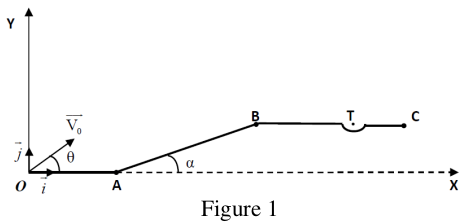
\includegraphics[width=0.6\textwidth]{./ex_05.png}
  \end{center}

Les points B, T et C sont alignés.
On néglige l’action de l’air et les dimensions de la balle. On prendra $g = 10 m.s^{-2}$.
L’étude du mouvement de la balle se fait dans un repère $(O,\vec{i}, \vec{j})$ lié à la terre et
supposé galiléen.

On lance, à l’instant $t = 0$, à
partir du point O, la balle vers le
trou T, avec une vitesse initiale
de valeur $V_0 = 10 m.s^{-1}$.

Le vecteur $\vec{V_0}$ est incliné d’un
angle $\theta$ = 45° par rapport à l’axe
horizontal (O,x).(Figure 1)

\begin{enumerate}
	\item Par application de la deuxième loi de Newton, établir les équations horaires
$x(t)$ et $y(t)$ du mouvement de la balle.
\item En déduire l’équation de la trajectoire de la balle.
\item Déterminer la valeur de xS, abscisse du sommet de la trajectoire de la balle.
\item  S’assurer que la balle passe au centre T du trou.
\end{enumerate}


\end{Box2}

%%_________________________Exercice 4 : _________________________Exercice
%\begin{Box2}{Exercice 7 :Le ski }
   %% \begin{wrapfigure}[12]{r}{0.5\textwidth}

%%\end{wrapfigure}


%\end{Box2}
\begin{center} \emph{\textbf{“It always seems impossible until it's done.”}}
\end{center}

%\vspace{-0.6cm}
%%%_________________________Exercice 5 : _________________________Exercice
%\begin{Box2}{Exercice 4 : }
   %% \begin{wrapfigure}[14]{r}{0.5\textwidth}
  %%\begin{center}
	  %%\vspace{-0.6cm}
	%%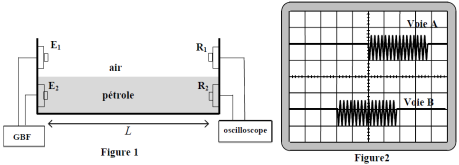
\includegraphics[width=0.5\textwidth]{./img/ex5.png}
  %%\end{center}
%%\end{wrapfigure}

%4

%\end{Box2}

%\begin{Box2}{Exercice 5 : }

%44
%\end{Box2}


%\begin{Box2}{Exercice 6 : }


	%\end{Box2}


%\begin{Box2}{Exercice 7 : }
%\end{Box2}
\end{document}
